% !TEX root = deckblatt3b.tex

\section{Nicht-Invertierender Verst\"arker}

In dieser Aufgabe sollte eine nichtinvertierende Operationsverstärkerschaltung aufgebaut und anschließend das Verhalten im
Gleich- und Wechselspannungsbetrieb ermittelt werden. Die Verstärkung war mit einem Faktor von 40-60 zu wählen.\\

\subsection{Schaltung}
\begin{figure}[H]
  \begin{center}
    %\tikzset{component/.style={draw,thick,circle,fill=white,minimum size =0.75cm,inner sep=0pt}}
    \resizebox{0.7\linewidth}{!}{
      \begin{circuitikz}
        \draw (0,0)
        (3,4) node[op amp,yscale=-1] (opamp) {}
        (3,4.5) to[short] (3,5) node[vcc] {$V_{CC}$}
        (3,3.5) to[short] (3,3) node[vss] {$V_{SS}$}
        (opamp.+) to[short] (0,4.5)
        (opamp.-) to[short] (1.5,3.5) to[short] (1.5,1.5) to[short] (4.5,1.5){}
        (4.5,4) to[R={$R_2$}] (4.5,1.5) to[R={$R_1$}] (4.5,-0.5) node[ground] (ground) {}
        (opamp.out) to[short] (8,4)
        (8,-0.5) node[ground] (ground) {}
        (0,-0.5) node[ground] (ground) {}
        ;
        \draw (0,4.2) to[short] (0,0.2) node[vee] {};
        \draw (-0.5,2.2) node[] {$U_e$};
        \draw (8,3.7) to[short] (8,0.2) node[vee] {};
        \draw (8.5,1.7) node[] {$U_a$};

      \end{circuitikz}
    }
    \caption{nicht inververtierender OPV}
  \end{center}
\end{figure}
\noindent
Der Operationsverstärker wurde mit $\pm15V$ versorgt und die Widerstände wurden wie folgt gewählt.\\
\begin{align*}
 R_1 &= 1k\Omega, R_2 = 47k\Omega\\
 \frac{U_a}{U_e} &= \frac{R_1 + R_2}{R_1}\\
 U_a &= U_e(1 + \frac{R_2}{R_1})\\
 U_a &= 48*U_e\\
\end{align*}

\subsection{Gleichspannungsverhalten}

Um das Verhalten im Gleichspannungsbetrieb zu ermitteln wurde der OPV zuerst mit einer Eingangsspannung von $100mV$ und anschließend
mit $300mV$ beaufschlagt.\\

\begin{table}[H]
\begin{minipage}{.5\textwidth}
\begin{figure}[H]
\centering
 \begin{tabular}{c|c}
  $U_e$ & $99,7mV$ \\ \hline
  $U_a$ & $4,8V$ \\ \hline
  $U_{R1}$ & $100mV$ \\ \hline
  $U_{R2}$ & $4,73V$ \\ \hline
  $U_d$ & $-0,5mV$ \\ \hline
  $I_{R1}$ & $0,096mA$ \\ \hline
  $I_{R2}$ & $0,101mA$ \\ \hline
  $I_+$ & $0mA$ \\ \hline
  $I_-$ & $0mA$ \\
 \end{tabular}
  \caption{Messwerte $0,1V$ DC}
\end{figure}
\end{minipage}
\begin{minipage}{.5\textwidth}
\begin{figure}[H]
  \centering
 \begin{tabular}{c|c}
  $U_e$ & $299mV$ \\ \hline
  $U_a$ & $14,21V$ \\ \hline
  $U_{R1}$ & $295mV$ \\ \hline
  $U_{R2}$ & $13,91V$ \\ \hline
  $U_d$ & $4,4mV$ \\ \hline
  $I_{R1}$ & $0,298mA$ \\ \hline
  $I_{R2}$ & $0,298mA$ \\ \hline
  $I_+$ & $0mA$ \\ \hline
  $I_-$ & $0mA$ \\
 \end{tabular}
 \caption{Messwerte $0,3V$ DC}
\end{figure}
\end{minipage}
\end{table}
\noindent
In den Messwerten kann man die lineare 48-fache Verstärkung der Eigangsspannung erkennen. Betrachtet man einen
idealen Operationsverstärker so sollten die Ströme an den Eingängen gleich null und die Spannung am Widerstand $R_1$
gleich der Eingangsspannung sein. Diese Annahme stimmt auch gut mit den Messwerten überein. Auch die Ströme an den
beiden Widerständen sind nahezu gleich groß, dies ist erforderlich um die Spannungsteilerregel in der Übertragungsfunktion
verwenden zu können.\\

\newpage
\subsection{Wechselspannungsverhalten}

Zum protokollieren des Wechselspannungsverhalten sollte ein Rechtecksignal an den OPV angelegt und dessen Frequenz variiert
werden.\\

\begin{figure}[H]
 \begin{center}
  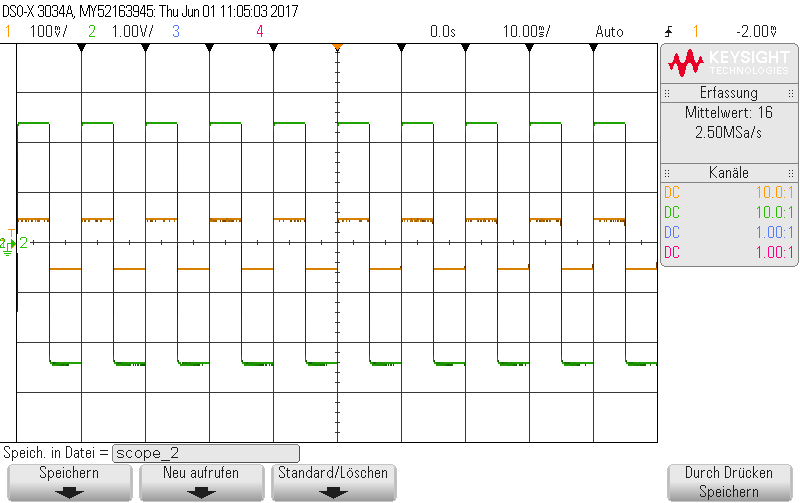
\includegraphics[height=6cm,width=12cm]{OsziBilder/nichtInvVer_100Hz}
 \end{center}
 \caption{Rechteckspannung $0,1V_{pp}$, $100Hz$ ($U_e$ orange, $U_a$ grün)}
\end{figure}

\begin{figure}[H]
 \begin{center}
  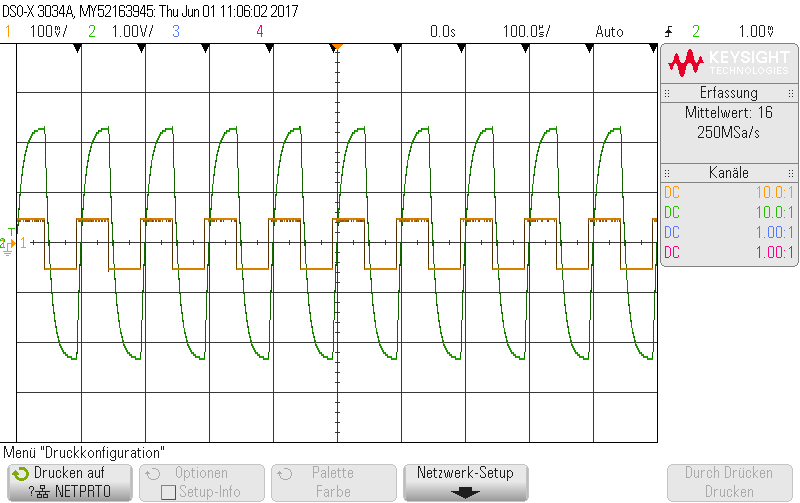
\includegraphics[height=6cm,width=12cm]{OsziBilder/nichtInvVer_10kHz}
 \end{center}
 \caption{Rechteckspannung $0,1V_{pp}$, $10kHz$ ($U_e$ orange, $U_a$ grün)}
\end{figure}
\noindent
Das $100Hz$ Signal zeigt eine schöne $1:48$ Übertragung. Bei $10kHz$ jedoch
wurde die Grenzfrequenz der Operationsverstärkerschaltung überschritten und das bauteilbedingte Tiefpassverhalten wirkt sich
auf die Ausgangsspannung aus. Daher wird das Signal nicht mehr im korrekten Verhältnis verstärkt und verschliffen übertragen.\\
